\section{Inter-Core Communication Protocol}

A critical challenge in implementing a software-defined GPU on a dual-core MCU is ensuring efficient and correct synchronization between the Control Unit (Core 0) and the Execution Units (Core 1). We employ a strictly ordered producer-consumer model using FreeRTOS primitives.

\subsection{Communication Mechanism}

The system relies on two primary queues:

\begin{enumerate}
    \item \textbf{Instruction Queue (\texttt{instrQueue})}: A deep buffer (size 64) that carries \texttt{InstrBatch} objects from Core 0 to Core 1. This allows the Front-End to "run ahead" of the Back-End, smoothing out fetch latencies.
    \item \textbf{Feedback Queue (\texttt{feedbackQueue})}: A small, high-priority queue used when Core 1 needs to report a predicate result back to Core 0 (e.g., for \texttt{BR.Z} or \texttt{OP\_BAR\_SYNC}).
\end{enumerate}

\subsection{Instruction Batching}

To reduce the overhead of context switching and queue locking, instructions are not sent individually. Instead, they are packed into \textbf{Instruction Batches}.

\begin{lstlisting}[language=C++]
struct InstrBatch {
    uint8_t count;          // 1-16 Instructions
    Instruction insts[16];  // Payload
    
    // Control Signals
    bool is_sync_req;       // Requires barrier?
    bool is_exit;           // End of Kernel?
};
\end{lstlisting}

Core 0 fills this batch until it encounters a control dependency (branch) or the batch is full. It then pushes the entire batch to the queue in a single operation.

\subsection{Synchronization Sequence}

Fig. \ref{fig:seq} illustrates the timing interaction during a typical execution flow involving a conditional branch.

\begin{figure}[htbp]
\centering
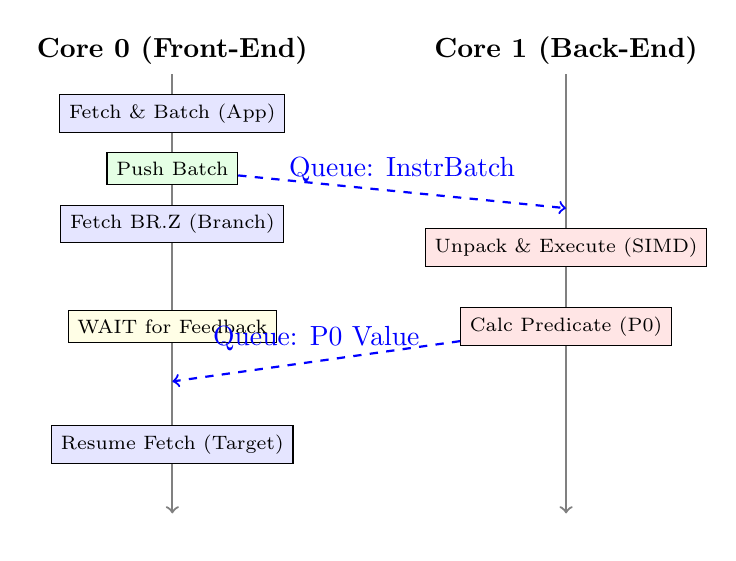
\begin{tikzpicture}[node distance=2cm, auto,
    timeline/.style={->, thick, gray},
    msg/.style={->, thick, blue, dashed},
    box/.style={rectangle, draw, fill=white, font=\scriptsize}]

    % Timelines
    \node (c0_top) at (0,0) {\textbf{Core 0 (Front-End)}};
    \node (c1_top) at (5,0) {\textbf{Core 1 (Back-End)}};
    \node (c0_bot) at (0,-6) {};
    \node (c1_bot) at (5,-6) {};

    \draw[timeline] (c0_top) -- (c0_bot);
    \draw[timeline] (c1_top) -- (c1_bot);

    % Sequence Steps
    
    % 1. Fetch
    \node[box, fill=blue!10] (f1) at (0, -0.8) {Fetch \& Batch (App)};
    
    % 2. Push Batch
    \node[box, fill=green!10] (push1) at (0, -1.5) {Push Batch};
    \draw[msg] (push1) -- node[above] {Queue: InstrBatch} (5, -2.0);
    
    % 3. C1 Execute
    \node[box, fill=red!10] (exec1) at (5, -2.5) {Unpack \& Execute (SIMD)};
    
    % 4. C0 continues fetching (Run Ahead)
    \node[box, fill=blue!10] (f2) at (0, -2.2) {Fetch BR.Z (Branch)};
    
    % 5. C0 waits for feedback
    \node[box, fill=yellow!10] (wait) at (0, -3.5) {WAIT for Feedback};
    
    % 6. C1 processes branch dependency
    \node[box, fill=red!10] (exec2) at (5, -3.5) {Calc Predicate (P0)};
    
    % 7. Feedback
    \draw[msg] (exec2) -- node[above] {Queue: P0 Value} (0, -4.2);
    
    % 8. Resume
    \node[box, fill=blue!10] (resume) at (0, -5.0) {Resume Fetch (Target)};

\end{tikzpicture}
\caption{Synchronization Sequence Diagram. Normal instructions are pipelined via batches. Control flow instructions (e.g., BR.Z) trigger a feedback loop, stalling Core 0 until Core 1 processes the predicate.}
\label{fig:seq}
\end{figure}

\subsubsection{Handling Divergence}
When Core 0 decodes a \texttt{BR.Z P0} instruction:
1. It flushes the current batch to Core 1 immediately.
2. It sends a special \texttt{SYNC\_REQ} signal.
3. It blocks on the \texttt{feedbackQueue}.
4. Core 1 executes all pending instructions, then reads the value of P0 from Lane 0 (or a consensus of lanes), and sends it back.
5. Core 0 receives the value, updates the PC, and resumes fetching.

This design ensures that control flow decisions are always based on the most up-to-date GPU state, preventing hazards.
